\documentclass[12pt,a4paper]{article}
\setlength\textwidth{145mm}
\setlength\textheight{247mm}
\setlength\oddsidemargin{15mm}
\setlength\evensidemargin{15mm}
\setlength\topmargin{0mm}
\setlength\headsep{0mm}
\setlength\headheight{0mm}
% \openright makes the following text appear on a right-hand page
\let\openright=\clearpage

%% Settings for two-sided (duplex) printing
% \documentclass[12pt,a4paper,twoside,openright]{report}
% \setlength\textwidth{145mm}
% \setlength\textheight{247mm}
% \setlength\oddsidemargin{14.2mm}
% \setlength\evensidemargin{0mm}
% \setlength\topmargin{0mm}
% \setlength\headsep{0mm}
% \setlength\headheight{0mm}
% \let\openright=\cleardoublepage

%% Character encoding: usually latin2, cp1250 or utf8:
\usepackage[utf8]{inputenc}


%% Further useful packages (included in most LaTeX distributions)
\usepackage{amsmath}        % extensions for typesetting of math
\usepackage{amsfonts}       % math fonts
\usepackage{amsthm}         % theorems, definitions, etc.
\usepackage{amssymb}	    % \Subset
\usepackage{bm}             % boldface symbols (\bm)
\usepackage{graphicx}       % embedding of pictures
\usepackage{fancyvrb}       % improved verbatim environment
\usepackage{dcolumn}        % improved alignment of table columns
\usepackage{booktabs}       % improved horizontal lines in tables
\usepackage{paralist}       % improved enumerate and itemize
\usepackage[pdftex,dvipsnames]{xcolor}  % typesetting in color


\usepackage{cite}
\usepackage[colorinlistoftodos,prependcaption,textsize=tiny]{todonotes}
\usepackage{xargs}
\usepackage{bbm}	% For lowercase blackboard bold
\usepackage{multicol}  	% ultiple columns
\usepackage{enumerate}


\newcommand{\R}{{\mathbb R^3}}

\newcommandx{\problem}[2][1=]{\todo[linecolor=red,backgroundcolor=red!25,bordercolor=red,#1]{#2}}
\newcommandx{\todoo}[2][1=]{\todo[linecolor=blue,backgroundcolor=blue!25,bordercolor=blue,#1]{#2}}
\newcommandx{\note}[2][1=]{\todo[linecolor=OliveGreen,backgroundcolor=OliveGreen!25,bordercolor=OliveGreen,#1]{#2}}
\newcommandx{\unsure}[2][1=]{\todo[linecolor=Plum,backgroundcolor=Plum!25,bordercolor=Plum,#1]{#2}}

\newtheorem{theorem}{Theorem}

\theoremstyle{definition}
\newtheorem{definition}{Definition}

\theoremstyle{remark}
\newtheorem{remark}{Remark}

\theoremstyle{theorem}
\newtheorem{proposition}{Proposition}


\newcommand{\tbd}{\textbf{{\color{red}~ TO BE DONE ~}}}

\newcommand{\x}{\mathbbm{x}}

\title{Existence of Gibbs distributions with Delaunay and Laguerre-Delaunay potentials}
\author{Daniel Jahn}

\begin{document}

\maketitle
\tableofcontents

\section{Notation, basic terms}
\todoo[inline]{Refer to remark 3.7 from \cite{DDG11} somewhere}

We will restrict ourselves to $(\mathbb R^3, \mathcal B)$, where $\mathcal B$ is the Borel $\sigma$-algebra on $\R$. Denote $\mathcal B_0 \subset \mathcal B$ the system of bounded Borel sets with positive Lebesgue measure, Denote $S$ the mark space with a Borel $\sigma$-algebra $\mathcal S$. In our case, $S = [0,W]$ for some $W>0$. A \textit{configuration} is a subset $\x \in \mathbb R^3\times S$ with a locally finite projection onto $\mathbb R^3$. Individual points from $\x$ will typically denoted $p=(p',p'')$ where $p' \in \mathbb R^3$ is called the \textit{center} of $p$ and $p'' \in S$ is called the \textit{weight} of $p$. Given the geometric interpretation (section \ref{sec:LD}),  the word \textit{point} and \textit{sphere} will be used interchangeably in this text.

Since this text also deals with the Delaunay triangulation, which does not take into account the marks, we will often tacitly identify a point $p'\in\R$ with the marked point $p=(p',0)$ with $p''=0$. In that sense, these ``unmarked'' points are still elements of $\R\times S$ and other terms do not have to be define twice for marked and unmarked configurations. We will use the word ``unmarked'' to mean \textit{with marks set to $0$}. \unsure{Once the text is finished, see how I used this notation and comment on it better.} 
% Sometimes it will be useful to denote that a whole configuration is unmarked in this manner. For that purpose we will use the notation $(\eta', \x')$. 

The space of all configurations on $\mathbb R^3 \times S$ is denoted $N$. It is equipped with the \todoo{Define the sigma algebra}standard $\sigma$-algebra $\mathcal N$. Let $N_f \subset N$ be the space of all configurations with finitely many points with the trace $\sigma$-algebra $\mathcal N_f$. For $\Lambda\in\mathcal B$ we write $\x_{\Lambda} = \x \cap (\Lambda \times S)$ and $N_\Lambda = \{\x \in N: \x = \x_\Lambda\}$, the set of configurations contained entirely in $\Lambda$, and write \todoo{The notation $\mathcal N'$ is problematic, since dash suggests unmarked point patterns} $\mathcal N'_\Lambda$ for the corresponding trace $\sigma$-algebra.

The reference measure on $(N, \mathcal N)$ is the Poisson point process $\Pi^z$ with intensity measure $z\lambda \otimes \mu$, where $z>0$ is called the \textit{activity}, $\lambda$ is the Lebesgue measure on $\mathbb R^3$ and $\mu$ is a $\sigma$-finite measure on $(S,\mathcal S)$. For $(N_\Lambda, \mathcal N_\Lambda)$, the reference measure will be $\Pi^z_\Lambda := \Pi^z \circ \text{pr}^{-1}_{\Lambda\times S}$, where $\text{pr}_{\Lambda \times S}$ denotes the projection onto $\Lambda \times S$.

\begin{definition}
	\begin{itemize}
		\item A \textit{hypergraph structure} is a measurable subset $\mathcal E$ of $(N_f\times N, \mathcal N_f \otimes \mathcal N)$ such that $\eta \subset \x$ for all $(\eta,\x)\in\mathcal E$. We call $\eta$ a \textit{hyperedge} of $\x$ and write $\eta \in \mathcal E(\x).$
		\item A \textit{hyperedge potential} is a measurable function $\varphi:\mathcal E\to \mathbb R \cup \{+\infty\}$. 
		\item Hyperedge potential is \todoo{Define $\vartheta_x$} \textit{shift-invariant} if 
			$$(\vartheta_x \eta, \vartheta_x \x) \in \mathcal E \text{ and } \varphi(\vartheta_x \eta, \vartheta_x \x) = \varphi(\eta,\x) \text { for all } (\eta,\x)\in\mathcal E \text{ and }x \in \R.$$
	\end{itemize}
\end{definition}

For notational convenience, we set $\varphi = 0$ on $\mathcal E^c$. 


\section{Delaunay and Laguerre-Delaunay hypergraph structures and potentials}
\subsection{Hypergraph structures}
\unsure[inline]{Do we actually need the normal position for points? All definitions work regardless}
The two key hypergraph structures used in this text are the Delaunay and Laguerre-Delaunay tetrahedronizations. 

\subsubsection{Delaunay hypergraph structure}
\begin{definition}
	We say that $(\eta,\x)$ satisfies the \textit{empty sphere property} if there exists an open ball $B(\eta,\x)$ with \note{Perhaps use $\x'$ for the point locations?}$B(\eta,\x)\cap \text{pr}_\R \x = \emptyset$ and $\eta \subset \partial B(\eta,\x) \cap \text{pr}_\R \x$. The sphere $\partial B(\eta,\x)$ \unsure{Maybe define $B(\eta,\x)$ before empty sphere, so it's always defined} is called the \textit{circumsphere}, the ball $B(\eta,\x)$ is the \textit{circumball}. 
\end{definition}
Note that the definition completely ignores the marks of $\x$, which are important only for the Laguerre-Delaunay case.

\unsure[inline]{Is $B(\eta,\x)$ even a good notation since for tetrahedra it does not depend on $\x$.}

\begin{definition}
The Delaunay hypergraph structure $\mathcal D$ is defined as
$$\mathcal D = \left\{ (\eta,\x) \in N_f \times N: \eta \subset \x, \# \eta = 4, (\eta,\x) \text{ satisfies the empty sphere property} \right\}. $$ 
\end{definition}

Note the differences from \cite{DDG12}, namely that we're only considering \textit{tetrahedral hyperedges}, i.e. hyperedges with four points, and that $\partial B(\eta,\x) \cap \x$ only needs to contain $\eta$ instead of being equal to it. This definition allows e.g. points in a regular lattice to still define tetrahedral hyperedges. In \cite{DDG12}, a regular lattice would still yield a nonempty hyperedge structure, but its hyperedges would not be tetrahedral. \unsure{Is this correct?}

\subsubsection{Laguerre-Delaunay hypergraph structure}\label{sec:LD}
In order to define the Laugerre-Delaunay hypergraph structure, we need to introduce further concepts.

\begin{definition}
Define the \textit{power distance} of the unmarked point $q' \in\R$ from the point $p=(p',p'') \in \R\times S$ as
$$d(q',p) = \|q'-p'\|^2 - p''.$$
\end{definition}

\begin{definition}
For two (marked) points $p=(p',p'')$ and $q=(q',q'')$, define their \textit{power product} by
$$\rho(p,q) = \|p'-q'\|^2 - p'' - q''.$$
Notice that $\rho(p,q) = d(p,q') - q'' = d(q,p') - p''$ and that $\rho(p,(q',0)) = d(p,q')$.
\end{definition}

\todoo[inline]{Talk about the geometric interpretation}
\begin{definition}
For a tetrahedral hyperedge $\eta$, we define the \textit{characteristic point} of $\eta$ as the point $p_\eta = (p'_\eta, p''_\eta)$ such that
$$\rho(p,p_\eta)=0 \text{ for all } p \in \eta.$$
\end{definition}
Note that the characteristic point can be thought of as a ball or sphere with the center $p'_\eta$ and radius $\sqrt{p''_\eta}$. This ball will be referred to as $B(p'_\eta,\sqrt{p''_\eta})$.

\todoo[inline]{Comment on uniqueness of this point - e.g. maybe we need to choose one with minimal weight}
\todoo[inline]{Again, talk about the geometric interpretation, orthogonality, etc.}

\begin{definition}
We say that $(\eta,\x)$ is \textit{regular} if $\rho(p_\eta,p)\geq 0 $ for all $p \in \x$.
\end{definition}

\todoo[inline]{Again, comment on the geometric interpretation of this property}

Using these terms, we are now ready to define the Laguerre-Delaunay hypergraph structure

\begin{definition}
	The Laguerre-Delaunay hypergraph structure $\mathcal {LD}$ is defined as 
	$$\mathcal {LD} = \left\{ (\eta,\x) \in N_f \times N: \eta \subset \x, \# \eta = 4, (\eta,\x) \text{ is regular } \right\}.$$
\end{definition}

\todoo[inline]{Titles for remarks (and maybe definitions too?)}

\begin{remark}[$\mathcal D$ as a special case of $\mathcal {LD}$] If all the points from $\x$ have weight 0, then the regularity property of $(\eta, \x)$ becomes the empty sphere property. Similarly, the characteristic point then coincides with the circumsphere. It would have therefore been possible to simply define $\mathcal D$ as a special case of $\mathcal {LD}$. We have decided to keep the definitions and related terms separate in order to stress the different properties of these two hypergraph structures. 
\end{remark}


\todoo[inline]{Finish these remarks}
\begin{remark}[Invariance in weights] \label{r:invariance} Tessellation is invariant in addition in weights $\Rightarrow$ Delaunay is obtained for any configuration with equal marks \tbd
\end{remark}

\begin{remark}[Redundant points]
	\tbd
\end{remark}

Since both of the hyperedge structures only contain tetrahedral edges, that is $\# \eta = 4$, we will tacitly assume any $\eta$ to be tetrahedral for the remainder of this text. 



\subsection{Hypergraph potentials}
Throughout this text, \note{For now}two potentials will mainly be used for both $\mathcal D$ and $\mathcal {LD}$. For a tetrahedral $\eta$, denote $\delta(\eta)=\text{diam}B(\eta,\x)$, the diameter of the circumsphere. 

% \problem[inline]{This is WRONG, since $p'_\eta$ depends on the marks, too, and won't be the same as the center of $B(\eta,\x)$. Is the assertion even true?}
% \begin{remark}
% 	For any $\eta=\{p_1,p_2,p_3,p_4\}$ and any $i=1,2,3,4$,  \todoo{Half diameter is an ugly notation for radius} we have
% 	$$p''_\eta = \|p'_\eta - p'_i\|^2 - p''_i \leq \|p'_\eta-p'_i\|^2 = 1/2\cdot \text{diam} B(\eta,\x)$$
% 	From this we can see two things. One, the diameter of the characteristic point is bounded by the diameter of the circumsphere. Two, their diameters equal only in the Delaunay case, that is if $p''_i=0$ for all $i=1,2,3,4$. 
% \end{remark}

\begin{definition}
	The \textit{smooth-interaction potential} $\varphi_S$ is a hyperedge potential satisfying $$\varphi_S(\eta,\x) \leq K_0 + K_1(\delta(\eta))^\beta$$for some $K_0 \geq 0, K_1 \geq 0, \beta > 0$.

	The \textit{hardcore interaction potential} $\varphi_{HC}$ for which there are constants $0\leq d_0 < d_1 \leq \alpha$ \unsure{How exactly does this look? Why?} such that
	$$\sup_{\eta: d_0 \leq \delta(\eta) \leq d_1} \varphi_{HC}(\eta,\x) < \infty \text{ and } \varphi_{HC}(\eta,\x)=\infty \text{ if } \delta(\eta)>\alpha.$$ 
\end{definition}
For simplicity, we assume that $\varphi_{HC}$ depends only on the points of $\eta$ in the sense of remark \ref{r:potential} below.

\problem[inline]{Define the dependence on $\eta$ clearly. Also the remark does not actually follow from the definition, since we're only bounding $\varphi_S$, it could still depend on neighbors}
\todoo[inline]{Talk a bit about $\varphi_{HC}$ - can be $\infty$ below $d_0$, requires infinity later,..}

\begin{remark}[Potentials' dependence on $\x$]\label{r:potential}
	The potentials depend on $\x \setminus \eta$ only in the sense that they equal to $0$ if $\eta \notin \mathcal E(\x)$. One implication of this is that the remaining points of $\x$ can never change the value $\varphi(\eta,\x)$ in other way than setting it to zero if $\eta \notin \mathcal E(\x)$. In other words, if $\eta \in \mathcal E(\x)$ and we take another configuration $\tilde{\x}$, then $\varphi(\eta,\tilde{\x}) \neq \varphi(\eta,\x)$ precisely only when $\varphi(\eta,\x) > 0$  and $\eta \notin \mathcal E(\tilde{\x})$, so that $\varphi(\eta,\tilde{\x})=0$.
\end{remark}

\todoo[inline]{Other potentials. Other characteristics other than circumdiameter. Combinations of potentials. Interaction.}
\tbd 

In the remainder of this text, whenever we say a property holds for $\mathcal D$ we mean that the property holds for the pair $(\mathcal D,\varphi_S)$ and $(\mathcal D,\varphi_{HC})$. Similarly for $\mathcal {LD}$ and $(\mathcal {LD},\varphi_S)$ and $(\mathcal {LD}, \varphi_{HC})$.




\section{Basic notions of hypergraph structures}

\begin{definition}
	A set $\Delta \in \mathcal B_0$ is a \textit{finite horizon} for the pair $(\eta,\x) \in \mathcal E$ and the hyperedge potential $\varphi$ if for all $\tilde{\x} \in N, \tilde{\x} = \x$ on $\Delta\times S$ 
$$(\eta,\tilde{\x})\in\mathcal E \text{ and } \varphi(\eta,\tilde{\x}) = \varphi(\eta,\x). $$
The pair $(\mathcal E, \varphi)$ satisfies the \textit{finite-horizon property} if each $(\eta,\x)\in \mathcal E$ has a finite horizon.
\end{definition}

The finite horizon of $(\eta,\x)$ delineates the region outside which points can no longer violate the regularity (or the empty sphere property) of $\eta$. 

\begin{remark} [Finite horizons for $\mathcal D$ and $\mathcal {LD}$]
For $\mathcal D$, the closed circumball $\bar B(\eta,\x)$ itself is a finite horizon for $(\eta,\x)$.

For $\mathcal {LD}$, the situation is slightly more difficult. For one, $B(p'_\eta, \sqrt{p''_\eta})$ does not contain the points of $\eta$. To see this, take two points $p,q$ with $p'',q''>0$ such that $\rho(p,q)=0$. Then $q'' = d(q',p) < \|q'-p'\|^2$ and thus $\sqrt{q''} < \|q'-p'\|$. More importantly, however, any point $s$ outside of $B(p'_\eta, \sqrt{p''_\eta})$ with a sufficiently large weight can violate the inequality $\rho(p_\eta,s) = \|p'_\eta - x'\|^2 - p''_\eta - s'' \geq 0$. 

To obtain a finite horizon for $\mathcal {LD}$, we need to use the fact that the mark space is bounded, $S=[0,W]$. If $s'' \leq W$, then $\Delta = B(p'_\eta, \sqrt{p''_\eta + W})$ is sufficient as a horizon, since any point $s$ outside $\Delta$ satisfies
$$\rho(p_\eta, s) = \|p'_\eta - s'\|^2 - p''_\eta - s'' \geq (\sqrt{p''_\eta+W})^2-p''_\eta-W = 0.$$ 

From a practical perspective, the maximum weight $W$ limits the resulting tessellation in the sense that the difference of weights can never be greater than $W$. Marks greater than $W$ are not necessarily a problem, as we can always find an identical tessellation with marks bounded by $W$, as long as there no two points $p,q$ with $|p''-q''|>W$ (see remark \ref{r:invariance}).
\end{remark} 

\todoo[inline]{Hamiltonians}
\begin{definition} Hamiltonian \tbd
\end{definition}

\todoo[inline]{Talk about $\x_{\Lambda^c}$ essentially being the boundary condition}
	
Next we must define the set of hyperedges $\eta$ in $\x$ for which either $\eta$ or $\varphi(\eta,\x)$ depends on $\x_\Lambda$.

\begin{definition} 
$$\mathcal E_\Lambda(\x) := \{ \eta \in \mathcal E(\x): \varphi(\eta,\zeta \cup \x_{\Lambda^c}) \neq \varphi(\eta,\x) \text{ for some } \zeta \in N_\Lambda \}$$
\end{definition}
\note[inline]{Later in the text, these are exactly the sets of tetrahedra used for the calculation, connect those two}

For $\mathcal D$, $\eta \in \mathcal D_\Lambda(\x)$ $\iff$ $B(\eta,\x) \cap \Lambda \neq \emptyset$. \newline
For \todoo{Explain why}$\mathcal {LD}$, $\eta \in \mathcal {LD}_\Lambda(\x) \iff d(p'_\eta,\Lambda) \leq \sqrt{p''_\eta + W}$, where \todoo{Confusing notation, $d$ is reserved for the power distance}$d(p'_\eta,\Lambda) = \inf\{\|p'_\eta - x\|: x \in \Lambda\}$ is the distance of $p'_\eta$ from $\Lambda$.    \newline

The final basic term again characterizes a type of finite-range property, this time as a property of the configuration $\x$.

\begin{definition}
	Let $\Lambda \in \mathcal B_0$ be given. We say a configuration $\x\ \in N$ \textit{confines the range of $\varphi$ from $\Lambda$} if there exists a set $\partial \Lambda(\x) \in \mathcal B_0$ such that $\varphi(\eta,\zeta \cup \tilde{\x}_{\Lambda^c}) = \varphi(\eta,\zeta\cup\x_{\Lambda^c})$ whenever $\tilde{\x} = \x$ on $\partial \Lambda(\x)\times S$, $\zeta \in N_\Lambda$ and $\eta \in \mathcal E_\Lambda(\zeta\cup\x_{\Lambda^c})$. In this case we write $\x \in N^\Lambda_\text{cr}$. We denote $r_{\Lambda,\x}$ the smallest possible $r$ such that $(\Lambda + B(0,r))\setminus \Lambda$ satisfies the definition of $\partial \Lambda(\x)$. We will use the abbreviation $\partial_\Lambda \x = \x_{\partial \Lambda(\x)}$.
\end{definition}

\todoo[inline]{Comment on the definition and what it means for $\mathcal D$ and $\mathcal {LD}$.}

\section{Existence assumptions and theorems}
We will now present the assumptions needed for the existence of the Gibbs measure.


\begin{enumerate}[\textbf{(R)}]
	\item \textit{Range condition}. There exist constants $\ell_R,n_R \in \mathbb N$ and $\delta_R < \infty$ such that for all $(\eta,\x) \in \mathcal E$ there exists a finite horizon $\Delta$ satisfying: For every $x,y \in \Delta$ there exist $\ell$ open balls $B_1, \dots, B_\ell$ (with $\ell \leq \ell_R$) such that
	\begin{enumerate}[-]
		\item the set $\cup^\ell_{i=1} \bar B_i$ is connected and contains $x$ and $y$, and 
		\item for each $i$, either $\text{diam} B_i \leq \delta_R$ or $N_{B_i}(\x) \leq n_R$.
	\end{enumerate}
\end{enumerate}

\subsection{Stability condition}
The second assumption is the well-known stability condition. 
\begin{enumerate}[\textbf{(S)}] 
	\item \textit{Stability}. The hyperedge potential $\varphi$ is called \textit{stable} if there exists a constant $c_S \geq 0$ such that 
$$H_{\Lambda,\x}(\zeta) \geq -c_S \#(\zeta \cup \partial_\Lambda \x)$$
for all $\Lambda \in \mathcal B_0, \zeta \in N_\Lambda, \x \in N^\Lambda_{\text{cr}}$.
\end{enumerate}

The first thing to note that when $\varphi$ is non-negative, then we can simply choose $c_S = 0$. The interesting cases therefore is when $\varphi$ can attain negative values.\newline

\subsubsection{Stability in $\mathbb R^2$}
In $\mathbb R^2$, the argument for stability of (Laguerre)-Delaunay hypergraph structures utilizes sublinearity of the hypergraph structure. We say that a hypergraph $\mathcal E$ is \textit{sublinear} if there exists $C < \infty$ such that $\# \mathcal E(\x) \leq C \# \x$ for all $\x \in N_f$. In the case of sublinearity of $\mathcal E$, it is sufficient that $\varphi$ is bounded from below, $\varphi \geq - c_\varphi$ for some $c_\varphi < \infty$, since then 
$$H_{\Lambda,\x} \geq -c_\varphi \#\mathcal E(\x) \geq -c_\varphi\cdot C \# \x$$ 
and thus $c_S = c_\varphi \cdot C$.

Sublinearity of any Laguerre-Delaunay triangulation in $\mathbb R^2$ is easily obtainable in at least two ways. One, using Euler's formula for planar graphs for the number of vertices ($v$), edges ($e$) and faces ($f$): $v-e+f=2$, which estabilishes a linear relationship between $v$ and $f$. Second, by a direct argument using the fact that any triangulation of $\mathbb R^2$ can be transformed into any other triangulation by a finite series of flips which do not change the number of triangles\cite{Lawson72}. A point inserted into the triangulation is located within a triangle $T$. Three new triangles within $T$ are then created and $T$ itself is removed. Any subsequent flips then leave the total number of triangles constant.\newline

\subsubsection{Stability in $\R$}
In $\R$, the situation is more difficult and neither of these approaches work. Any graph can be embedded in $\R$\cite{3dGraph} and thus an analog to Euler's formula in three dimensions cannot exist, as it would have to characterize any finite graph. The number of tetrahedra also no longer remains constant under topological flipping\cite{Joe91}. 

This is no wonder - it is well known (see e.g. \cite{Amenta07}) that the complexity\footnote{For our purposes, we can define complexity as the number of tetrahedra in the tessellation.} of the Delaunay tetrahedronization of $n$ points is $\mathcal O(n^2)$ in general. However, this result is not yet dooming to the stability of the Gibbs models. For one, all the known example of point configurations that attain the upper complexity bound are distributed on one-dimensional curves such as the \textit{moment curve}\cite{Amenta07}. In fact, in \cite{Erickson01}, Erickson states that ``For all practical purposes, three-diimensional Delaunay triangulations appear to have linear complexity.''. While hardly a proof, this is encouraging to anyone wishing to simulate Delaunay models with potentials that can attain negative values.

More importantly the fact that Delaunay tetrahedronization  can have $\mathcal O(n^2)$ tetrahedra \textit{in general} does not mean that this is the case for the Poisson-Delaunay tetrahedronization, i.e. Delaunay tetrahedronization of a configuration generated by a Poisson point process. If the Poisson-Delaunay tetrahedronization of $n$ points have $\mathcal O(n)$ tetrahedra almost surely, then the Gibbs-Delaunay tetrahedronization would inherit this property by absolute continuity. Dwyer \cite{Dwyer93} proved that the expected number of tetrahedra is $\mathcal O(n)$. More recently, Erickson has provided \cite{Erickson01}\cite{Erickson05} complexity bounds based on a characteristic of a configuration called \textit{spread}, defined as the ratio between the longest and shortest pairwise distance. Delaunay tetrahedronization of point configuration with spread $\Delta$ has complexity $\mathcal O(\Delta^3)$. This is a hopeful result, since the spread of point configurations is loosely connected with its dimensionality, in that e.g. regular lattice of in $\mathbb R^d$ with $n$ points has spread $\mathcal O(n^{1/d})$.\todoo{Make this more precise} Values such as the nearest neighbor distance are easily tractable with the Poisson process, giving a chance to a simple solution to the stability question. However, to the best of our knowledge, the current literature does not directly give an answer to this problem.

\todoo[inline]{Simulation study}

For now, assume that all potentials used in this text are non-negative.

\subsection{Upper regularity}

In order to present the upper regularity conditions, we introduce the notion of \textit{pseudo-periodic} configurations. 

Let $M\in\mathbb R^{3\times 3}$ be an invertible $3\times 3$ matrix with column vectors $(M_1,M_2,M_3)$. For each $k \in \mathbb Z^3$ define the cell
$$C(k) =  \{Mx \in \R: x-k \in \left[ -1/2, 1/2 \right)^3 \}.$$
These cells partition $\R$ into parallelotopes. We write $C=C(0)$. Let $\Gamma \in \mathcal N'_C$ be non-empty. Then we define the \textit{pseudo-periodic} configurations $\bar \Gamma$ as
$$\bar \Gamma = \{ \x \in N: \vartheta_{Mk}(\x_{C(k)}) \in \Gamma \text{ for all } k \in \mathbb Z^3 \},$$
the set of all configurations whose restriction to $C(k)$, when shifted back to $C$, belongs to $\Gamma$. The prefix pseudo- refers to the fact that the configuration itself does not need to be identical in all $C(k)$, it merely needs to belong to the same class of configurations.

\begin{enumerate}[\textbf{(U)}] 
	\item \textit{Upper regularity}. $M$ and $\Gamma$ can be chosen so that the following holds. 
		\begin{enumerate}[(U1)]
			\item \textit{Uniform confinement}: $\bar \Gamma \subset N^\Lambda_\text{cr}$ for all $\Lambda \in \mathcal B_0$ and 
			$$r_\Gamma := \sup_{\Lambda\in\mathcal B_0}\sup_{\x \in \bar\Gamma} r_{\Lambda, \x} < \infty$$
			\item \textit{Uniform summability}: 
			$$c^+_\Gamma := \sup_{\x \in \bar\Gamma}  \sum_{\eta \in \mathcal E(\x): \eta \cap C \neq \emptyset} \frac{\varphi^+(\eta,\x)}{\#(\hat\eta)} < \infty,$$
where $\hat\eta := \{k \in \mathbb Z^3: \eta \cap C(k) \neq \emptyset\}$ and $\varphi^+ = \max(\varphi,0)$ is the positive part of $\varphi$.
\item \textit{Strong non-rigidity}: $e^{z|C|} \Pi^z_C(\Gamma) > e^{c_\Gamma}$, where $c_\Gamma$ is defined as in (U2) with $\varphi$ in place of $\varphi^+$.
		\end{enumerate}
\end{enumerate}


\problem[inline]{The remark is wrong in general (in particular finitely many summands don't imply finite supremum, and indeed that's not the case here), have this only after introducing $\Gamma^A$}
\begin{remark}[(U2)]\label{r:U2}
	For $\mathcal D$ and $\mathcal {LD}$ it always holds that $\#\{\eta \in \mathcal E(\x): \eta \cap C \neq \emptyset\}<\infty$. Therefore the only quantity in (U2) which could be infinite is $\varphi^+(\eta,\x)$ and the condition reduces to $\varphi^+(\eta,\x) <  \infty$. This then means that the condition (U2) is non-trivial only for hardcore-interaction models.
\end{remark}

\todoo[inline]{Remark about U3 monotonicity, possibly some other remarks about the assumptions}

\todoo[inline]{Get more intuition about U3 and comment on why \^U is useful}

For some models it is possible to replace the upper regularity assumptions by their alternative and prove the existence for all $z>0$.

\begin{enumerate}[(\textbf{\^{U}})]
	\item \textit{Alternative upper regularity}. $M$ and $\Gamma$ can be chosen so that the following holds.
	\begin{enumerate}[(\^U1)]
		\item \textit{Lower density bound}: There exist constants $c,d > 0$ such that $\#(\zeta) \geq c|\Lambda| - d$ whenever $\zeta \in N_f\cap N_\Lambda$ is such that $H_{\Lambda,\x}(\zeta)<\infty$ for some $\Lambda \in \mathcal B_0$ and some $\x \in \bar\Gamma$.
		\item = (U2) \textit{Uniform summability}.
		\item \textit{Weak non-rigidity}: $\Pi^z_C(\Gamma) > 0$.
	\end{enumerate}
\end{enumerate}

\todoo[inline]{Define Gibbs measure}

\begin{theorem}
	For every hypergraph structure $\mathcal E$, hyperedge potential $\varphi$ and activity $z>0$ satisfying \textbf{(S)}, \textbf{(R)} and \textbf{(U)} there exists at least one Gibbs measure.
\end{theorem}

\begin{theorem}
	For every hypergraph structure $\mathcal E$, hyperedge potential $\varphi$ and activity $z>0$ satisfying \textbf{(S)}, \textbf{(R)} and \textbf{(\^{U})} there exists at least one Gibbs measure.
\end{theorem}







\subsection{$M$ and $\Gamma$ for Laguerre-Delaunay models}\label{sec:MGamma}
For the Delaunay and Laguerre-Delaunay models, the choice of $M$ and $\Gamma$ will be the following. Fix some $A \subset C\times S$ and define
$$\Gamma^A = \{\zeta \in N_C: \zeta = \{p\}, p \in A\},$$
the set of configurations consisting of exactly one point in the set $A$.

Let $M$ be such that $|M_i| = a > 0$ for $i=1,2,3$ and $\measuredangle(M_i,M_j) = \pi / 3$ for $i\neq j$.\todoo{Comment better on why this choice}

In \cite{DDG12}, $A$ is chosen to be $B(0,b)$ for \unsure{$\rho_0$ possibly conflicts with $\rho$ for the power product}$b\leq \rho_0 a$ for some \unsure{The vagueness about $\rho_0$ is not satisfactory, though it's the way DDG did it. If possible, change this} sufficiently small $\rho_0 >0$. We will use this form as well - the question, however, is how to choose the mark set. It would be convenient to choose $A=B(0,b)\times\{w\}$ for some $w\in S$ and then only deal with a Delaunay triangulation, but this \problem{Only true if $\mu$ is non-atomic. But we could use an atomic $\mu$ for working with Delaunay.} would mean that $\Pi^z_C(\Gamma) = 0$, conflicting with both $(U3)$ and $(\hat U3)$. The choice $A=B(0,b)\times S$ could, for a small enough $a$, result in some spheres being fully contained in their neighboring spheres, possibly resulting in redundant points, thus changing the desired properties of $\Gamma$. It is thus necessary to choose the mark space dependent on $a$. For given $a,\rho_0$, the minimum distance between individual points is $a-2\rho_0 a = a(1-2\rho_0)$. We therefore choose $A = B(0,b)\times [0, \sqrt{\frac a2(1-2\rho_0)}]$ in order for spheres to never overlap \unsure{This is perhaps unnecessarily conservative, we could widen it}. 

\begin{remark}[Simplification of (U2) and (U3)]\label{r:UA}
	Using the set $\Gamma^A$, we can simplify the assumptions (U2) and (U3).
	
	For (U3), we can now directly calculate $\Pi^z_C(\Gamma)$.
	\begin{align*} 
		\Pi^z_C(\Gamma) &= \Pi^z_C(\{\zeta \in N_C: \zeta = \{p\}, p \in A\}) \\
		& = e^{-z|A|} z |A| e^{-z|C\setminus A|} \\
		& = e^{-z|C|} z |A|,
	\end{align*}
	and thus (U3) becomes
	$$z|A| > e^{c_{A}},$$
	where $c_A := c_{\Gamma^A}$.

	In the case $A = B(0,\rho_0 a)\times [0, \sqrt{\frac a2(1-2\rho_0)}]$, we have
	$$|A| = \frac 43 \pi (\rho_0 a)^3 \cdot \sqrt{\frac a2(1-2\rho_0)} = \frac {4\pi}{3\sqrt{2}}\cdot  \rho_0^3 \sqrt{1-2\rho_0} \cdot a^{7/2}$$

	For (U2), we obtain the simplification $\#(\hat\eta) = \#\eta$, since now each point of $\eta$ is necessarily in a different set $C(k)$.
\end{remark}

\todoo[inline]{Number some equations for reference}


\subsubsection{Geometrical structure of the tessellation defined by $M$ and $\Gamma^A$}
\todoo[inline]{Better description and arguments of nearly everything in this section}
In order to be able to check the assumptions of the existence theorems, we must investigate the structure of the tessellations formed from $\bar\Gamma^A$ further. Namely there are two main quantities of interest, both coming from the term $c_A$:
\begin{enumerate}
	\item The number of tetrahedra incident to the point in $C$,  
		$$n_T := \# \{\eta \in \mathcal E(\x): \eta \cap C \neq \emptyset\}.$$
	\item The behaviour of the hyperedge potentials $\varphi_{S}$ and $\varphi_{HC}$ for $\eta \in \mathcal {LD}(\x)$ and $\x \in \Gamma^A$.
\end{enumerate}

Let $\x' \in \Gamma_A$ be such that each point is in the center of $A$ with marks set to $0$. In $\mathbb R^2$, such configuration generates a tessellation composed of equilateral triangles with side lengths $a$. In $\R$, the situation is more complex. The vectors $M_1,M_2,M_3$ do in fact form a regular tetrahedron, as all its faces are necessarily equilateral triangles, but the entire tesselation cannot be composed of merely regular tetrahedra, as they alone do not tessellate, as Aristotle famously claimed\cite{Lagarias12}. To be able to characterize the tessellation $\mathcal {LD}(\x')=\mathcal D(\x')$, it will be useful to use a concrete example of the matrix $M$:

$$
\begin{pmatrix}
1 & \frac 12 & \frac 12 \\
0 & \frac {\sqrt{3}}2 & \frac 1{2\sqrt{3}}  \\
0 & 0 & \sqrt{\frac 23} \\
\end{pmatrix}.
$$

Under this transformation the points of the unit cube get mapped in the following way:

$$\begin{matrix}
	p_1: & (0,0,0) & \rightarrow & (0,0,0) \\
	p_2: & (1,0,0) & \rightarrow & (1,0,0)\\
	p_3: & (0,1,0) & \rightarrow & (1/2,\sqrt{3}/2,0)\\
	p_4: & (1,1,0) & \rightarrow & (3/2,\sqrt{3}/2,0)\\

	p_5: & (0,0,1) & \rightarrow & (1/2,1/(2\sqrt{3}),\sqrt{2/3})\\
	p_6: & (1,0,1) & \rightarrow & (3/2,1/(2\sqrt{3}),\sqrt{2/3})\\
	p_7: & (0,1,1) & \rightarrow & (1,2/\sqrt(3), \sqrt{2/3})\\
	p_8: & (1,1,1) & \rightarrow & (2,2/\sqrt(3), \sqrt{2/3})\\
\end{matrix}$$

If we connect all the nearest-neighbors, we will obtain a tessellation of $\R$. The resulting structure is that of two regular tetrahedra ($p_1,p_2,p_3,p_5$ and $p_4,p_6,p_7,p_8$) and a regular octahedron ($p_2,\dots ,p_7$), which are well known to tessellate\footnote{ The tessellation is of great importance to many fields and thus is known under many names. In mathematics, it is most commonly called the \textit{tetrahedral-octahedral honeycomb}, or the \textit{alternated cubic honeycomb}. In structural engineering, it is known as the \textit{octet truss}, as named by Buckminster Fuller, or the \textit{isotropic vector matrix}. It is stored as \textit{fcu} in the Reticular Chemistry Structure Resource\cite{RCSR}. It is also the nearest-neighbor-graph of the face-centered cubic (fcc) crystal in crystallography\cite{Gabbrielli12}.  }. Figure \ref{fig:explode} shows an exploded view of the resulting tessellation and figure \ref{fig:tetra-oct} shows the cell $C$ with the two tetrahedra and one octahedron outlined. 


\begin{figure}
  \centering
  \begin{minipage}{0.45\textwidth}
	  \centering
	  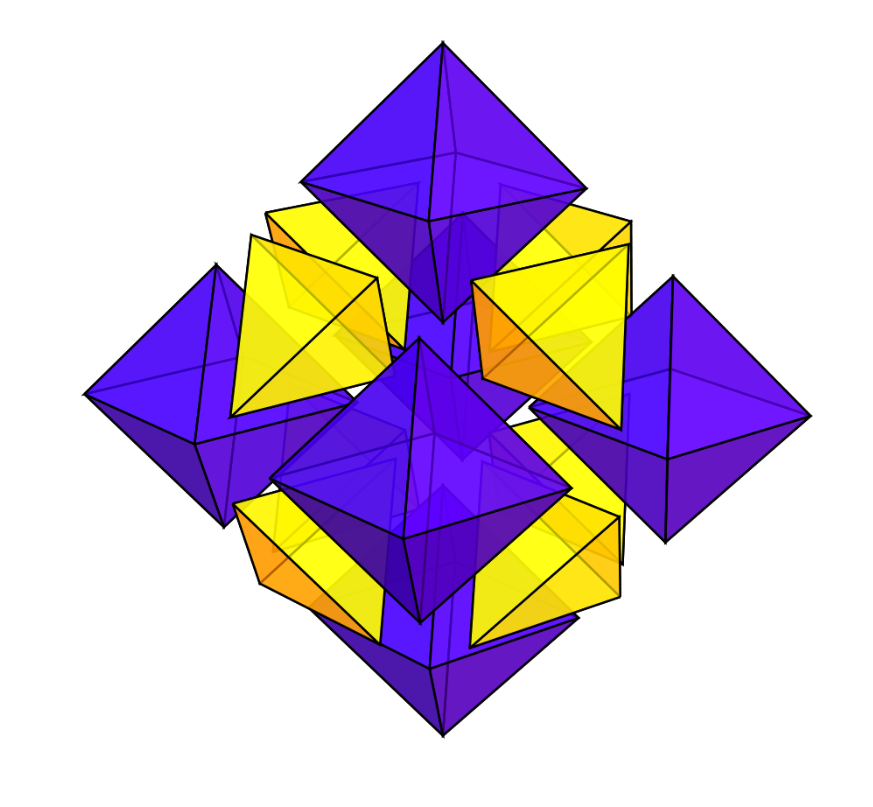
\includegraphics[width=1\textwidth]{Figures/tetra-exploded.PNG}
	  \caption{The tessellation in an exploded view.}
	  \label{fig:explode}
  \end{minipage}\hfill
  \begin{minipage}{0.45\textwidth}
	  \centering
	  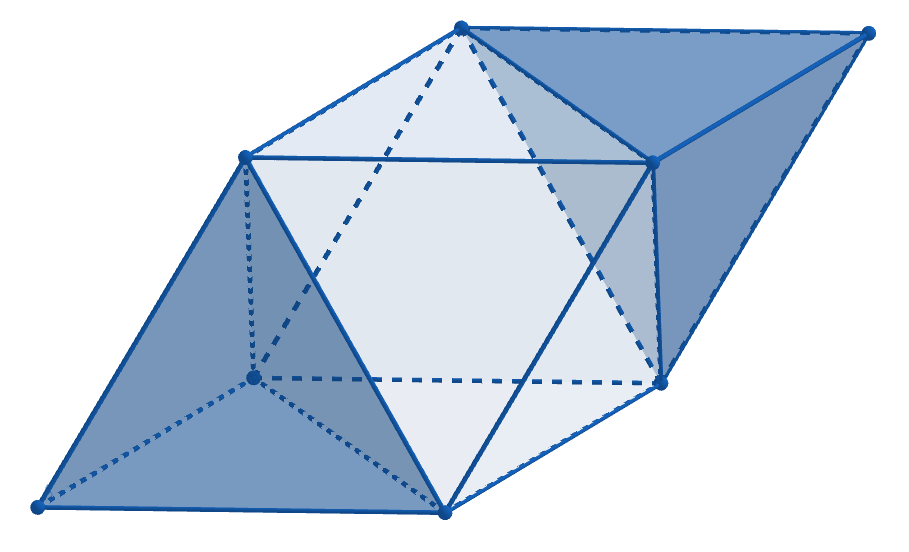
\includegraphics[width=1\textwidth]{Figures/tetra-tess.png}
	  \caption{The set $C$ tessellated by two tetrahedra and an octahedron.}
	  \label{fig:tetra-oct}
  \end{minipage}
\end{figure}


% tikz http://www.texample.net/tikz/examples/parallelepiped/
% Each point has 12 NN, all at the same distance
% http://cosmometry.net/vector-equilibrium-&-isotropic-vector-matrix


However, this tessellation is not yet a Delaunay tetrahedronization, as we still have to tetrahedronize the regular octahedron $O=(p_2,\dots, p_7)$. A regular octahedron is a Platonic solid an as such all of its vertices are cocircular. As a result, all of $\binom{6}{4}=15$ \problem{Not true, coplanar points don't} quadruples form a tetrahedron, resulting in a degenerate case which is nevertheless alowed in our definition of $\mathcal D$. \todoo{This is an important point, probably come back to it later. It's quite likely it will be possible to turn this into a formal argument..} In most (in fact almost surely w.r.t. $\Pi^z$) configurations in $\Gamma^A$ this won't be the case as the tetrahedron won't be regular. However, since we're interested in the supremum, we must consider this extreme case.

In $\mathcal D(\x')$, we therefore have two types of tetrahedra. The first is the regular tetrahedron itself. The second is the tetrahedron used to tessellate the octahedron with all side lengths equal to $a$ except for the diagonal which is equal to $\sqrt{2}a$.

% All the tetrahedra
% {a, b, c, d} plane
%{a, c, e, f} plane
%{b, d, e, f} plane 
%
%{a, b, c, e} {a, c, d, e}
%{a, b, c, f} {a, c, d, f}
%
%{a, b, d, e} {b, c, d, e}
%{a, b, d, f} {b, c, d, f}
%
%{a, b, e, f} {a, d, e, f}
%{b, c, e, f} {c, d, e, f} 

The circumdiameter of each of the tetrahedra can be \note{Possibly comment on this more} calculated by imagining an additional vertex equidistant from the vertices of the tetrahedron and setting the Cayley-Menger determinant\cite{Cayley1841}\cite{Menger28}\footnote{A nice derivation in English can be found in \cite{Uspensky48}. It turns out that the Cayley-Menger determinant is basically derived from squaring the INCIRCLE determinant used to calculate the circumcenter.} equal to zero. This gives the results $\sqrt{6}/4 \cdot a$ for the regular tetrahedron and $1/\sqrt{2} \cdot a$ for the other tetrahedron.

\todoo[inline]{Most importantly: what is the supremum of the potential over $\x \in \bar\Gamma^A$?}
\tbd

Now we turn to the combinatorial structure of $\mathcal D(\x)$. In the tetrahedronized regular octahedron, each vertex is incident to $\binom{5}{3}=10$ tetrahedra. In the tetrahedron-octahedron tessellation, each \todoo{Reference, possibly using Schlafli symbols} vertex is incident to eight regular tetrahedra and six regular octahedra. This gives us $n_T = 8 + 6\cdot 10 = 68$. While still large, this is less than quarter of $8\cdot \binom{7}{3} = 280$ for the case of regular cube tessellation induced by the choice $M=aE$. Note that $n_T$ is much smaller for the non-degenerate case, when $O$ contains only $4$ tetrahedra and its vertices are incident either to $2$ or $4$ tetrahedra. In this case, $n_T\leq 8+6\cdot 4 = 32$.


\section{Checking the assumptions for our models}

\todoo{It might be useful to have such a general theorem anyway, but formulated properly} Until the exact bounds for $\varphi_S$ over $\bar\Gamma^A$ are found, it will be more illustrative to use a universal unary $\varphi_U(\eta,\x)=f(\eta)$, where $f$ is nonnegative and finite and e.g. equal to or bounded by (a power of, etc.) circumradius, volume, surface area, sum of edge lengths, \dots

\problem[inline]{It's nonsense to have to include the mark set, it only increases the bound for $z$}
\begin{proposition}
	The exists at least one gibbs measure for the model $(\mathcal D,\varphi_U)$ and every activity
	$$z > \frac{3\sqrt{2}}{4\pi \cdot \rho_0^3 \sqrt{1-2\rho_0}} e^{17 \varphi_{\text{max}}(a_{\text{min}})} / {a_{\text{min}}}^{7/2}.$$
\end{proposition}
\begin{proof}
\begin{enumerate}[]
	\item \textbf{(R)} The finite-horizon $\Lambda = \bar B(\eta,\x)$ with $\ell_R = 1, n_R = 0$ and $\delta_R$ arbitrary can be used. This is because it itself contains no points of $\x$ by definition of $\mathcal D$ and acts as the open ball from the definition of the range condition.
	\item \textbf{(S)} Stability is satisfied because of $\varphi$ is non-negative.
	\item \textbf{(U)} We choose $M$ and $\Gamma$ as in section \ref{sec:MGamma}.
		\begin{enumerate}[(U1)]
			\item For a small enough $\rho_0$, such that any three points in $\bar \Gamma$ cannot be coplanar, the class $\bar\Gamma$ provides an upper bound $d_{\text{max}}$ for $\text{diam} B(\eta,\x)$ for all $\eta \in \mathcal D(\x)$ for all $\x \in \bar \Gamma$ and we have $r_{\Gamma^A} \leq d_{\text{max}} $. \todoo{Talk about this more clearly} 
			\item Is trivially satisfied since $n_T < \infty$ and $\varphi(\eta,\x)<\infty$ for all $(\eta,\x)\in\mathcal D$ (see remark \ref{r:U2}).
			\item Using remark \ref{r:UA}, we want to find $z$ as small as possible such that $z|A| > e^{c_{\Gamma^A}}$. We can bound $c_{\Gamma^A} \leq \frac {n_T}4 \varphi_{\text{max}}(a) $ where $\varphi_{\text{max}}(a) = \sup_{(\eta,\x) \in D} \varphi_U(\eta,\x)$ where $D=\{ (\eta,\x): \x \in \bar\Gamma^A, \eta \in \mathcal D(\x): \eta\cap C \neq \emptyset\}$.  This gives us the bound
				\begin{equation}z > K e^{\frac{n_T}{4} \varphi_{\text{max}}(a)}/a^{7/2}\label{eq:prop1z}\end{equation}
				where $K = \frac{3\sqrt{2}}{4\pi \cdot \rho_0^3 \sqrt{1-2\rho_0}}$ and $n_T = 68$. We then find $a_\text{min}$ that minimizes the right-hand-side of \ref{eq:prop1z}.
		\end{enumerate}
\end{enumerate}
\end{proof}



\begin{proposition}
	The exists at least one gibbs measure for the model $(\mathcal D,\varphi_{HC})$ and every activity $z>0$.
\end{proposition}
\begin{proof}
\begin{enumerate}[]
	\item \textbf{(R)} Again, $\Lambda = \bar B(\eta,\x)$ with $\ell_R = 1, n_R = 0$. Because of the hard-core condition, we can also take $\delta_R = 2\alpha$.
	\item \textbf{(S)} Stability is satisfied because of $\varphi$ is non-negative.
	\item \textbf{(\^{U})} We choose $M$ and $\Gamma$ as in section \ref{sec:MGamma}.
		\begin{enumerate}[(\^{U}1)]
			\item \todoo{Again, this is very vague. Make the argument using exact expressions and the fact that regular tetrahedron minimizes the circumdiameter.} The fact that the circumdiameter is limited enforces a minimum density of points.
			\item \todoo{Vague, improve} is satisfied as long as we choose $a$ such that $1/\sqrt{2} a$ is much smaller than the maximum circumradius $\alpha$ (see remark \ref{r:U2}).
			\item $\Pi^z_C(\Gamma)>0$ due to the calculation in remark \ref{r:UA}.
		\end{enumerate}
\end{enumerate}
\end{proof}




\begin{proposition}
	The exists at least one gibbs measure for the model $(\mathcal {LD},\varphi_S)$ and every activity
	$$z > ?$$
\end{proposition}
\begin{proof}
\begin{enumerate}[]
	\item \textbf{(R)} Take the horizon set $\Delta = B(p'_\eta, \sqrt{p''_\eta + W})$. $\Delta$ can be decomposed into the sphere $p_\eta$ and $\Delta \setminus p_\eta$, a 3-dimensional annulus with width $\sqrt{p''_\eta+W} -\sqrt{p''_\eta}=W/(\sqrt{p''_\eta+W} + \sqrt{p''_\eta})$. By definition of $\mathcal {LD}$ and remark, $p_\eta$  cannot contain any points of $\x$. \todoo{Ugly line placements, improve} Although the annulus $\Delta \setminus p_\eta$ does not have any bound on the number of points, its width is bounded by $\sqrt W \geq  W/(\sqrt{p''_\eta+W} + \sqrt{p''_\eta})$. This means that any $x,y\in \Delta$ can be connected by the spheres $B(x,\sqrt W), p_\eta, B(y,\sqrt W)$, yielding the parameters $\ell_R = 3,n_R=0,\delta_R=2\sqrt W$.
	\item \textbf{(S)} Stability is satisfied because of $\varphi$ is non-negative.
	\item \textbf{(U)} We choose $M$ and $\Gamma$ as in section \ref{sec:MGamma}.
		\begin{enumerate}[(U1)]
			\item \todoo{Vague, improve} Similarly to proposition 1, as long as $\rho_0$ is small enough for any three points to never be coplanar, the weight $p''_\eta$ of the characteristic point is bounded and therefore also $r_\Lambda,\x$ is bounded for all $\Lambda \in \mathcal B_0$ and all $\x \in \bar \Gamma$.
			\item is trivially satisfied since $n_T < \infty$ and $\varphi(\eta,\x)<\infty$ for all $(\eta,\x)\in\mathcal {LD}$ (see remark \ref{r:U2}). 
			\item \tbd (..as soon as I have bounds on $\varphi_S$, calculation is otherwise simple and is outlined in Proposition 1)
		\end{enumerate}
\end{enumerate}
\end{proof}




\begin{proposition}
	The exists at least one gibbs measure for the model $(\mathcal {LD},\varphi_{HC})$ and every activity $z>0$.
\end{proposition}
\begin{proof}
\begin{enumerate}[]
	\item \textbf{(R)} The horizon set is $\Delta = B(p'_\eta,\sqrt{p''_\eta +W})$. Parameters can be chosen as in proposition 3. \unsure{Is it a problem that there's no $n_R$ circle? Cause the proof suggested something like that?}
		% Alternatively we have $ \sqrt{p''_\eta} \leq \alpha/2$ because of the hard-core condition, and thus we can also use $\ell_R = 1, \delta_R = 2 \sqrt{\alpha^2 + W}$ with $n_R$ arbitrary. 
	\item \textbf{(S)} Stability is satisfied because of $\varphi$ is non-negative.
	\item \textbf{(\^{U})} We choose $M$ and $\Gamma$ as in section \ref{sec:MGamma}.
		\begin{enumerate}[(\^{U}1)]
			\item \todoo{Vague, improve} The fact that the circumdiameter is limited enforces a minimum density of points.
			\item \todoo{Vague, improve} is satisfied as long as we choose $a$ such that $1/\sqrt{2} a$ is much smaller than the maximum circumradius $\alpha$ (see remark \ref{r:U2}).
			\item $\Pi^z_C(\Gamma^A) >0$ due to the calculation in remark \ref{r:UA}.
		\end{enumerate}
\end{enumerate}
\end{proof}


\bibliographystyle{unsrt}
\bibliography{bibliography-exist}

\listoftodos
\end{document}
